\documentclass[12pt]{article}
\usepackage{amsmath,amsthm,amssymb,dsfont,polynom}
\usepackage[pdftex]{graphicx}

\graphicspath{{images/}}

\usepackage{tikz}
\usepackage{ dsfont}
\usetikzlibrary{arrows}

\usepackage[margin = 1.0in]{geometry}
\usepackage{fancyhdr}
\usepackage{hyperref}
\pagestyle{fancy}
\lhead{Francis Pich\'e}

\thispagestyle{empty}


\newtheorem{problem}{Problem} 
\theoremstyle{definition} 
\newtheorem*{solution}{Solution}

\usepackage{listings}
\usepackage{color}

\definecolor{dkgreen}{rgb}{0,0.6,0}
\definecolor{gray}{rgb}{0.5,0.5,0.5}
\definecolor{mauve}{rgb}{0.58,0,0.82}

\lstset{frame=tb,
  language= Python,
  aboveskip=3mm,
  belowskip=3mm,
  showstringspaces=false,
  columns=flexible,
  basicstyle={\small\ttfamily},
  numbers=none,
  numberstyle=\tiny\color{gray},
  keywordstyle=\color{blue},
  commentstyle=\color{dkgreen},
  stringstyle=\color{mauve},
  breaklines=true,
  breakatwhitespace=true,
  tabsize=3
}


\begin{document}
\title{COMP 421 Study guide}
\author{Francis Pich\'e}
\date{\today}
\maketitle
\newpage
\tableofcontents
\newpage

\part{Preliminaries}
\section{Disclaimer}
These notes are curated from Joseph D'silva COMP421 lectures at McGill University. They are for study purposes only. They are not to be used for monetary gain.

\part{Introduction to Databases}
\section{Data Storage}
In operating systems, file systems are used for persistent storage. This is insufficient because:
\begin{itemize}
	\item Only provides a basic API
	\item Information may not be structured.
	\item Only linear seek possible (slow)
	\item May have data loss in case of power outages etc
	\item Can't have concurrent access to files
\end{itemize}

\section{Relational Model and Data Definition Language}
Entity Relationship Model is a language that describes the data determined through requirement analysis. This is very similar to UML, but is not the same. 
\subsection{Requirement Analysis}
When designing a database, we must first identify which data needs to be stored, and how it will be used. (Which operations need to be executed on the data).
\\ \linebreak
For example, if we were designing a database for Minerva at McGill, we would need to think about which entities are relevant to be stored. In OOP, these would be the classes. Things like the students, addresses, fees, courses etc are all relevant information. We would also need to think about the types of operations that must be possible by our database. Things like adding students, changing addresses, assessing fees etc.
\\ \linebreak
In an OOP setting, we would break down the problem by identifying classes and relationships between them. For example, we might have Student and Instructor classes, with a parent class Person, since the Student and Instructor share some attributes (name, age...). We also have relationships between classes such as a Student and Transcript. A Transcript does not exist unless assigned to a Student. We need ways to model all of these relationships in a database setting rather than an OOP setting.
\\ \linebreak
\subsection{ER}
An \textit{entity} is a real world object which contains a set of attributes. A collection of instantiated entities would be an \textit{entity set}. An entity set must have a \textit{key}. This is an attribute that is underlined, and MUST be unique. There can be two attributes underlined, in which case both COMBINED must be unique. Individually they need not be unique. 
\\ \linebreak
ISA ("is a") hierarchy is similar to subclasses in OOP. This is represented as a triangle. The key is still in the parent entity set. 
\\ 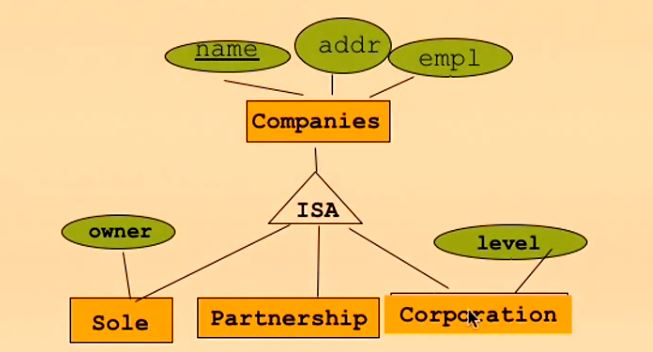
\includegraphics{isa}\\
There is a subtle point here in that unlike OOP, the attributes of the parent are not part of the child entity set (to avoid duplication, and keep things consistent).
\\ \linebreak
 If there are overlaps (a company can be both a partnership and Corporation), we must put a note explaining the situation. We assume that the parent is not covering all possible subtypes. (There may exist a company which is not a Sole, Partnership or Corporation).

\subsection{Relationships}
A relationship is an association among two or more entities. This can be one to one, many-to-one, many-to-many. A relationship set is a collection of similar relationships.
\\ \linebreak
There cannot be duplicate association instances. For example, if a Company donates 10\$ to a Party, (the association being the sponsorship), then there cannot be another 10\$ donation with the same Company and Party. The original must be updated.
\\ \linebreak
There are constraints as well.
We can add an arrow, or two, to constrain to a one-to-many or one-to-one (respectively).  
\\ 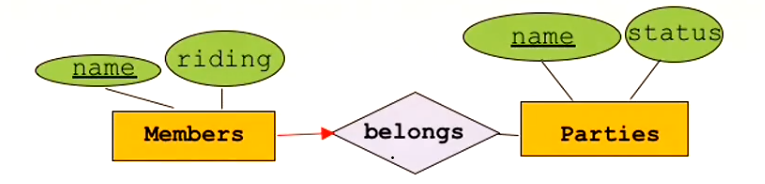
\includegraphics{one-to-many}
\\ 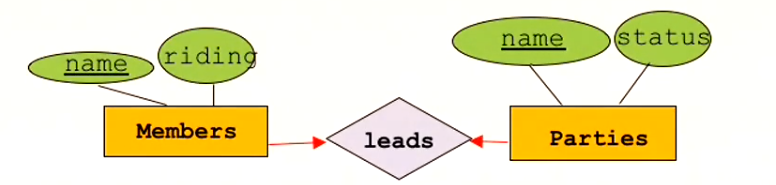
\includegraphics{one-to-one}\\
\textbf{Participation constraints} are when we must have at least one entity set is participating in the relationship.
\\ 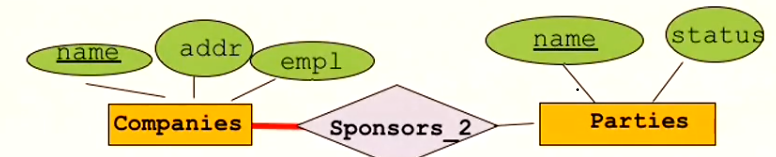
\includegraphics{at-least-one}\\
which is shown by a bold line. This can be combined with a key constraint to show a relationship in which exactly one entity set is related. 
\\ \linebreak
\textbf{Ternary relationships} are relationships involving 3 entity sets. Keep in mind that a ternary relationship database entries MUST include all 3 entities. If you have more than a ternary relationship (n-ary), it's probably an indication of bad design.
\\ \linebreak
\subsection{Weak Entities}
\textbf{Weak Entities} are entities which do not have a natural attribute which can be used as a key, but there is another entity set with which we can identify the entities. For example, suppose we have Teams and Players. The teams have names, Players have names and shirt numbers. Here, the Team name may be unique for a league, but not overall, and a shirt number may be unique within a team, but not for the league. However, we can use the Team name as a primary key, with the Player shirt number as a partial key to identify a player. Note that this implies that a Player cannot exist without belonging to a Team.
\\ 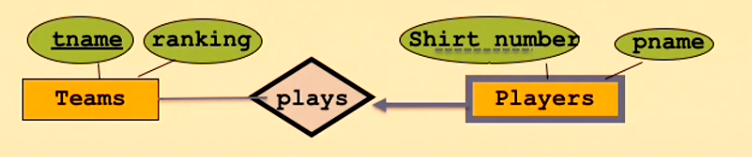
\includegraphics{weak-entity}\\
We often create artificial keys to keep track of information. For example student numbers. However, you should never use an artificial key as a partial key. If you're going to make one, make sure it's unique.
\\ \linebreak
We use weak entities when there is no global authority that allows creating unique identifiers.
\\ \linebreak
\subsection{Avoiding Redundancies}
We should avoid redundancies by not storing the same information more than once. This is important since it may allow for data to become out of sync. 
\\ 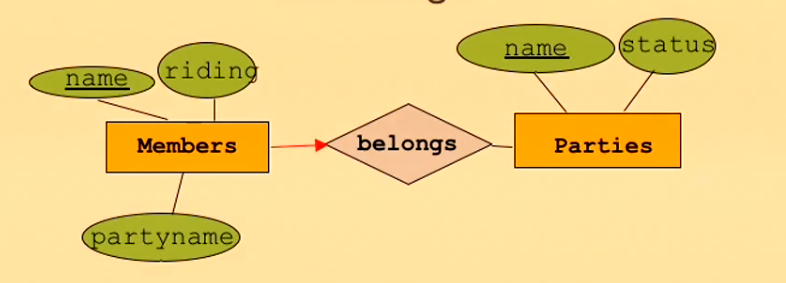
\includegraphics{redundant}\\
suppose someone changed the partyname but not the name of the associated party. The data would be inconsistent.
\\ \linebreak

\subsection{Entity Set or Attribute}
When can an entity set simply be an attribute? If we only care about the key of an entity set, and we only have a one to many relationship, we can represent it instead as an attribute. The one-to-many is important since we can't have a list as an attribute value. For example, if we have Movies, with the attribute Category (rather that have a relationship between Movie and Category), we can't have a list of Categories if the Movie belongs to several Categories. This would require leaving it as a relationship rather than an attribute.
\\ \linebreak

\section{Relational Model}
This is the most common model, and is closer to actual implementation. Used by iBM DB2, PostgreSQL, MySQL, SQLite etc.
\\ \linebreak
There are other types of models, which we will either ignore or look at later. 
\\ \linebreak
A relational database is nothing more than a set of relations. A relation consists of a schema and instance. A schema defines the name of a relation, its attributes, and the domain/type of each attribute. \texttt{Students(sid: int, name: string, login: string, faculty: string, major: string)} Ie: relation == table. Not to be confused with relationship in ER modeling (different things!). The instances are actual tuples (rows) in the table. 
\\ \linebreak
We cannot have identical instances (duplicate rows), at least one attribute value must be different. We also cannot assume anything about the order of the rows. The column order also doesn't matter. 
\\ \linebreak
\subsection{DDL and DML}
DDL (data definition language) defines the schema of a database. (What the tables are called, their attributes) This only gives structure, no real data.
\\ \linebreak
DML (data manipulation language) manipulates the data. (deals with instances of the relations). For example, insert, update delete, query etc.
\\ \linebreak

\section{Translating from ER to DDL}
Entity sets are easy, just use the name of the entity set and its attributes.
\texttt{EntitySetName(attr1: type,  attr2: type ... attrn: type)}
\\ \linebreak
\subsection{Relationships}
What if there is a relationship? Well first translate the entity sets involved, then the relationship is a relation with the key of each entity set as it's key, and then it's attributes.
\subsection{Key Constraints}
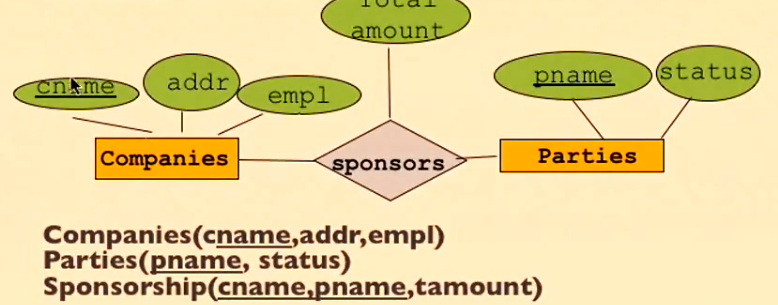
\includegraphics{translate}\\
What if there are key constraints?
For a one to many relationship, we can make the primary key to be only the key of one entity set.
\\ 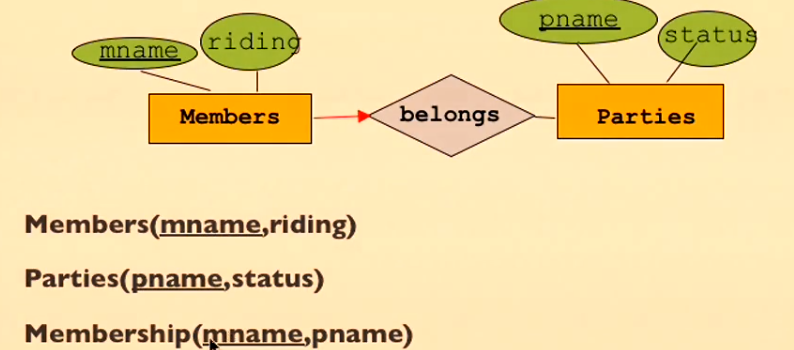
\includegraphics{key-constraint}\\
So here, we cannot have one member belonging to multiple parties in both the ER and the DDL (since mname must be unique in a table, and the key constraint is in the diagram). \
\\ \linebreak
We can actually do better here. By moving the pname attribute up into the Members table as an attribute, we can reduce the total number of tables by 1. (Eliminating the need for the Membership table). However, this is only good if all members will have a party. If the new column we created in Members is sparse (a lot of NULL's) then its a big waste of space, in which case the 3 table approach is better.
\\ \linebreak
\subsection{Participation Constraints}
Participation restraints are generally enforced by a NOT NULL on the foreign key. If we have a participation constraint on a key constraint, our 3 table solution from before no longer works. We now need to go with the 2 table solution since there is no way to enforce that the Members table has a corresponding entry in the Membership table (separate tables).
\\ \linebreak
If there is no key constraint along with the participation constraint (just the participation constraint on its own)\textbf{ THERE IS NO WAY TO ENFORCE IT.} It's an important note that \textbf{all} many-to-many relationships require 3 tables. And since participation constraints require 2 tables. So we must put a note to indicate that it should be a participation constraint.
\\ \linebreak

\subsection{Weak Entity Sets}
Translating weak entity sets requires both the partial key of the weak entity set, and the key of the entity set on which the weak depends on. 

\subsection{ISA Hierarchies}
For ISA, we need to copy the key of the parent into all child tables, and then just the attributes of each child.
\\ \linebreak
There is another way which is to copy ALL parent attributes and then add the child-specific attributes. This might lead to duplication, but also make things easier on an application/efficiency level.
\\ \linebreak
A last alternative is to have only a table for the root (parent) entity set, with attributes for all the attributes contained in all the children, with NULL's if the entry does not have that datatype. This easy to store, but requires a lot of care in the application, since there is nothing stopping NULL values to be updated with real values, causing inconsistency with the model. 
\\ \linebreak

\part{SQL}
SQL is used as a standard to define DDL and DML. There are many dialects of it in various DB's.
\\ \linebreak
SQL has data types.
\begin{itemize}
	\item CHAR (fixed length string)
	\item VARCHAR (variable length string with upper limit)
	\item INT
	\item SHORTINT
	\item FLOAT
	\item DOUBLE PRECISION
	\item DECIMAL (how many decimals are needed. )
	\item DATE
	\item TIME
\end{itemize}

\section{Creating a Table}
Very similar to DDL, just:
\begin{lstlisting}
CREATE TABLE students
	(sid INTEGER,
	 name VARCHAR(30),
	 login VARCHAR(30),
	 faculty VARCHAR(30),
	 major VARCHAR(30) DEFAULT 'undefined')
\end{lstlisting}
Note that the types are specified, it is case insensitive (but uppercase on commands is convention) and we can define default values.
\section{Simple Queries}
\subsection{Insert}
\begin{lstlisting}
INSERT INTO Students
	VALUES (53666, 'Bartoli', 'bartoli@cs', 
		    'Science', 'Software Engineering')
\end{lstlisting}
Note that the order of the values is the same as the order of our CREATE TABLE statement. If we want to insert only a subset of the values, we must specify which attributes are inserting. The rest will be NULL or default.
\begin{lstlisting}

INSERT INTO Students (sid, name, faculty)
VALUES (53668, 'Chang', 'Eng')
\end{lstlisting}

\subsection{Delete}
Similar syntax to Insert, but we need to specify a key on which to delete entries. 
\\ \linebreak
\begin{lstlisting}
DELETE
FROM Students
WHERE name = 'Chang'
\end{lstlisting}
This will delete all entries with the name as Chang. Any attribute can be used, or even a combination of attributes. 

\subsection{Update}
\begin{lstlisting}
UPDATE Students
SET major = 'Software Engineering'
WHERE sid = 53688
\end{lstlisting}
This will update the major of the entry with sid = 53688. We can update multiple columns at once as well the same way we inserted multiple values.

\section{Advanced Queries}

\section{Constraints}
We can use NOT NULL when defining the table to ensure that an attribute is non-empty.
\\ \linebreak
\subsection{Primary Key Constraints}
A set of fields is a \textbf{key candidate} if this set is unique in the table, and it is not true for any subset of the key set. Ie if there is a simpler unique key set, you must use it. If there are more than one elements in the set, then one is chosen to be a \textbf{primary key}.
\\ \linebreak
Often, this primary key is required to be NOT NULL. 
\subsection{Foreign Key}
A foreign key is a set of attributes from one relation that is used to refer to a tuple in another relation. 
\\ 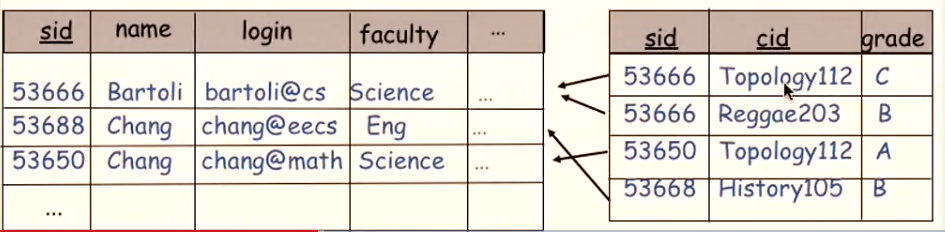
\includegraphics{foreign-key} \\
So here, sid refers to the students table, (foreign key) while the cid is the primary key of the Enrollment table. The foreign key must  be the primary key of the other table. However, if we delete a record from the student table, we must first delete all dependent records in the Enrollment table.
\begin{lstlisting}
CREATE TABLE Enrolled
(
	sid CHAR(9),
	cid VARCHAR(20),
	grade CHAR(2),
	PRIMARY KEY (sid, cid),
	FOREIGN KEY (sid) REFERENCES Students
)
\end{lstlisting}
\section{Application Programming}

\part{DB Internals}
\section{Buffer Management}
\section{Indexing}
\section{Query Execution}
\section{Query Optimization}
\section{KV Stores}
\section{Map Reduce}
\section{Transactions}
\section{Concurrency Control}
\section{New Trendy Stuff}

\end{document}